\section{Benchmark Variance}
A \nth{3} analysis is done on the Benchmark data to assess the variances of each of the benchmarks evaluated. To achieve this, a single nETL task is run to load a database with Benchmarks data for all students who attended CSC1015F in either 2014, 2015, or 2016 (or attended the course multiple times). The JSON used for configuring nETL to load data from the \texttt{Benchmarks (2014 - 2016).csv} file into CouchDB is included in the appendix at \ref{netl-task-6-config}, which is identical to the configuration of the Task 1 nETL process (except that a different database is used).

Following loading of the data from the CSV into CouchDB, a Map function is used to produce an index of the CouchDB documents sorted by Student ID. Only the single value (Student ID) is used for the key since the Map function only outputs a single document type no joining is required - in fact, since the results of this analysis is the coefficient of variation for each used benchmark, a List function is not required at all. Instead the coefficient of variation of each benchmark analyzed is read directly from the MapReduce output (i.e. the view-index).

\subsection{Map Function}
The map function for this analysis is included in the appendix (see \ref{variance-map-function}). Each document passed to the map function is treated according to the logic shown in the activity diagram in Figure \ref{fig-variance-map-function}. On Map function execution the ``type\_'' attribute is checked. If the document is not of type ``benchmark'', Map function execution is terminated, otherwise benchmarks are retrieved from the document, averages of combined benchmarks are calculated, and a tuple of the form \mintinline{text}{[StudentId: [benchmarks]]} is output by the Map function.

Similarly to other Map function processing of benchmark documents, a normalization of grade symbols to percentages is performed via a nested function within the Map function, and according to the logic as discussed previously and shown in in Table \ref{tbl-benchmarks-normalize}. However, Unlike with previous analyses, integer-based calculations are performed in the JavaScript code during Map function execution. All numbers in JavaScript are 64-bit Floating Point following the IEEE 754 standard \cite{floatingPoint}, with observed peculiarities when working with rational numbers with decimal points as a result. Due to the nature of how floating point arithmetic differs from base-10 arithmetic, rounding errors such as the example $0.1 + 0.2 = 0.30000000000000004$ need to be dealt with (or at least quantified). In this project the problem is sidestepped due to it's complicated nature \cite{Goldberg1991}, and an open source \nth{3}-party library (\texttt{decimal.js} \cite{decimaljs}) is used for handling arithmetic in the Map function instead. CouchDB supports the commonJS specification for module loading of JavaScript libraries in the context of Map function execution \cite{commonJsMapFn}.


\begin{figure}[H]
    \centering
    \begin{mdframed}
        \centering
        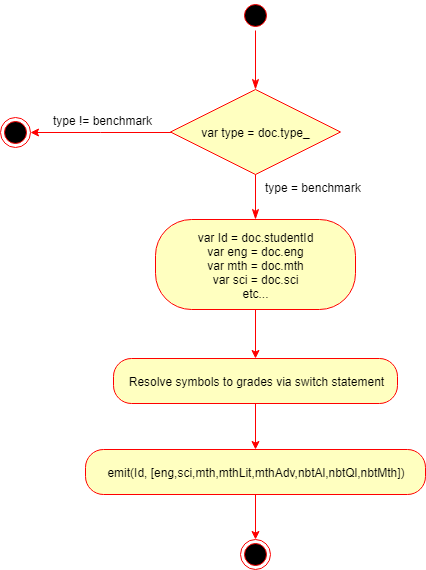
\includegraphics[scale=0.35]{./resources/figures/variance-map.png}
    \end{mdframed}
    \caption[Variance Map Function]{\textbf{Figure \ref{fig-variance-map-function}: Map function logic required for the variance analysis.} This logic is applied to every document during index calculation (excluding documents with an \_id of ``\_design/*''). The logic used to normalize grades-as-symbols to percentages is shown in Table \ref{tbl-grades-normalize} for the Grades data, and \ref{tbl-benchmarks-normalize} for the Benchmarks data.}
    \label{fig-variance-map-function}
\end{figure}